\subsection{Aufbau}
Das Toolkit ist in zwei Teile unterteilt (siehe Abbildung \ref{fig:mlagents_aufbau}). Für die Unity-Integration ist das Paket com.unity.ml-agents aus dem Unity Asset Store zuständig. Das eigentliche Training mit den maschinellen Lernalgorithmen findet jedoch in einer separaten Python-Umgebung statt. Für die Kommunikation zwischen den beiden Bereichen verwendet das ML-Agents Toolkit eine gRPC-Netzwerkkommunikation.\cite{juliani2020}

\begin{figure}[H]
  \centering  
  \begin{tikzpicture}[node distance=2cm]
  \node [rounded, draw=green, fill=green!30] (unity) {Unity Umgebung};
  \node [rounded, draw=red, fill=red!30, below of=unity] (python) {Python Umgebung};
  
  \draw [latex-latex, line width=0.3mm] (unity) -- (python);
  \end{tikzpicture}
  \caption{Unity ML-Agents Aufbau}
  \label{fig:mlagents_aufbau}
\end{figure}

Um eine Szene in Unity für das verstärkende Lernen zu nutzen muss die Szene mindestens ein Agent beinhalten. Jeder Agent referenziert ein Verhalten. Ein Verhalten kann eins von drei verschiedenen Modi verwenden. In Abbildung \ref{fig:mlagents_aufbau_unity} werden drei Agenten mit allen unterschiedlichen Verhalten Modi dargestellt.

\begin{figure}[H]
  \centering  
  \begin{tikzpicture}[node distance=2cm]
  
    \node (agent1) [rounded, draw=green, fill=green!30] {Agent 1};
    \node (agent2) [rounded, right of=agent1, xshift=2cm, draw=green, fill=green!30] {Agent 2};
    \node (agent3) [rounded, right of=agent2, xshift=2cm, draw=green, fill=green!30] {Agent 3};
    
    \node (verhalten1) [rounded, below of=agent1 , draw=yellow, fill=yellow!30] {Verhalten Lernen};
    \node (verhalten2) [rounded, below of=agent2 , draw=yellow, fill=yellow!30] {Verhalten Inferenz};
    \node (verhalten3) [rounded, below of=agent3 , draw=yellow, fill=yellow!30] {Verhalten Heuristik};

    \node (kommunikator) [rounded, below of=verhalten1, draw=orange, fill=orange!60] {Kommunikator};
    \node (sentis) [rounded, below of=verhalten2, draw=orange, fill=orange!50] {Sentis};
    \node (heuristik) [rounded, below of=verhalten3 , draw=orange, fill=orange!30] {Heuristik};
    
    \draw [latex-latex, line width=0.3mm] (agent1)  -- (verhalten1);
    \draw [latex-latex, line width=0.3mm] (agent2)  -- (verhalten2);
    \draw [latex-latex, line width=0.3mm] (agent3)  -- (verhalten3);

    \draw [latex-latex, line width=0.3mm] (verhalten1)  -- (kommunikator);
    \draw [latex-latex, line width=0.3mm] (verhalten2) -- (sentis);
    \draw [latex-latex, line width=0.3mm] (verhalten3) -- (heuristik);
    
  \end{tikzpicture}
  \caption{Unity ML-Agents Aufbau Unity Umgebung}
  \label{fig:mlagents_aufbau_unity}
\end{figure}

Das lernende Verhalten nutzt den Kommunikator um Beobachtungen an die Python Umgebung zu übergeben. Als Antwort bekommt das Verhalten die Aktion entnommen der aktuellen Strategie. Im Inferenz Modus wird ein bereits trainiertes Modell mit dem Unity Sentis Packet ausgeführt. Der Heuristik Modus wird meist zum testen oder dem Aufzeichnen von Demonstrationen für das Imitationslernen verwendet. Die Heuristik verwendet fest codierte Anweisungen um beispielsweise die Aktionen über Tastatureingabe zu steuern.

\begin{figure}[H]
  \centering  
  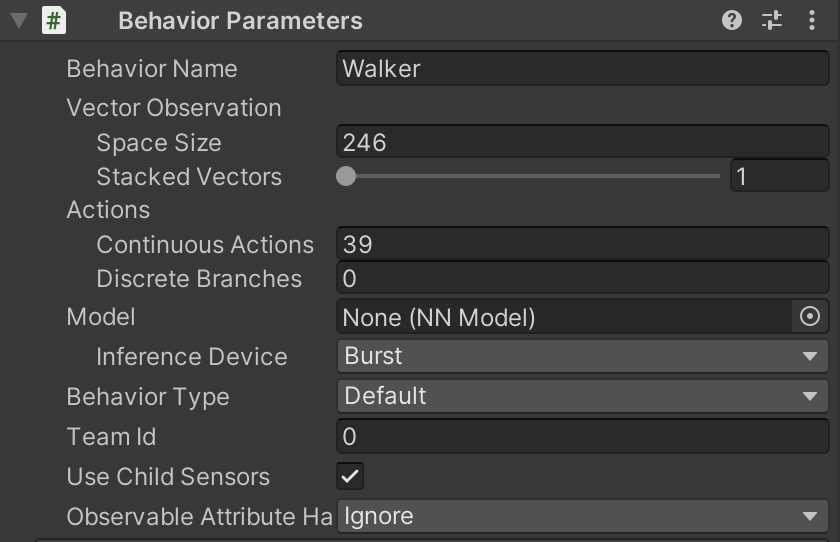
\includegraphics[scale=0.5]{img/verhalten_komponente.png}
  \caption{Unity ML-Agents Verhalten Parameter Komponente}
  \label{fig:verhalten_komponente}
\end{figure}

\begin{itemize}
  \item Behaviour Name: Name des Verhaltens / wird in Trainer Konfiguration referenziert
  \item Space Size: Anzahl an Beobachtungen / Inputknoten für NN
  \item Continuous Actions: Anzahl an Aktionen / Outputknoten von NN
  \item Model: Referenz auf bereits trainiertes Modell zur Verwendung in Inferenz
  \item Behaviour Type: Lernmodus Default = Lernen, Heuristic, Inferenz
\end{itemize}

Die Agent-Komponente bildet die Grundlage für alle Implementierungen. Sie bietet abstrakte Funktionen für die Initialisierung, den Start einer Episode, das Erfassen des Zustands der Umgebung sowie das Ausführen von Aktionen. Durch die Implementierung dieser Funktionen können unterschiedlichste Agenten entwickelt und trainiert werden. Die Beobachtungen des Agenten können auf zwei Arten erstellt werden. Beobachtungen basierend auf Raycasts sowie Kamerabildern werden mit seperate Komponenten erstellt. Beobachtungen aus Zahlenwerte sowie Vektoren und Quaternionen können jedoch auch direkt über die Observations Funktion im Agenten der Beobachtung angehängt werden.

\begin{figure}[H]
  \centering
  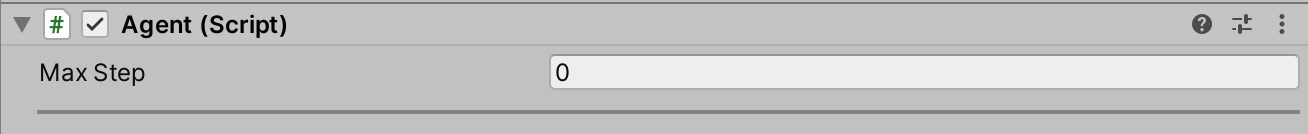
\includegraphics[scale=0.5]{img/agent_komponente}
  \caption{Unity ML-Agents Agenten Komponente}
  \label{fig:agent_komponente}
\end{figure}

Abbildung \ref{fig:agent_komponente} zeigt die Basiskomponente des Agenten. Die Agenten Komponente stellt alle grundlegenden Funktionen des verstärkenden Lernens bereit und implementiert die Verbindung zur Akademie und dem Verhalten des Agenten. Ohne das überschreiben der Funktionen ist die Agentenklasse jedoch ohne Funktion. Die genauen Methoden zur Implementierung eigener Agentenklassen werden im folgenden Abschnitt behandelt. Das einzige Feld zur Konfiguration ist Max Step, welches die maximale Anzahl der Schritte innerhalb einer Episode festlegt.

\begin{lstlisting}[caption={Agent Funktionen},captionpos=b,label={lst:agent_funktionen}]
public override void CollectObservations(VectorSensor sensor)
{
    sensor.AddObservation(floatObservation);
}

public override void OnActionReceived(ActionBuffers actionBuffers)
{
    var continuousActions = actionBuffers.ContinuousActions;
    movement.x += continuousActions[0]
    movement.y += continuousActions[1]
}

public virtual void FixedUpdate()
{
    AddReward(floatReward);
}
\end{lstlisting}

In der CollectObservations Methoden wird festgelegt welche Daten dem Agent für das Training bereit stehen siehe Listing \ref{lst:agent_funktionen} Zeile 1-3. CollectObservations wird für jede angefragte Entscheidung ausgeführt und das Ergebnis an das NN Modell oder den Python Trainer übergeben.

Wenn eine Entscheidung angefragt wurde und das NN Modell ein Ergebnis liefert wird dieses hier von numerischen Werten in Aktionen umgewandelt. In Listing \ref{lst:agent_funktionen} Zeile 6-11 wird gezeigt wie die Aktion in x und y Bewegung umgesetzt wird.

Im Beispielcode in Listing \ref{lst:agent_funktionen} Zeile 13-16 wird ein Reward in jedem FixedUpdate vergeben über die AddReward Methode die auch Teil der Agenten-Komponente ist. Der Reward kann aber an jeder Stelle im Code vergeben werden, der Code dient hier nur als ein Beispiel.

\begin{figure}[H]
  \centering  
  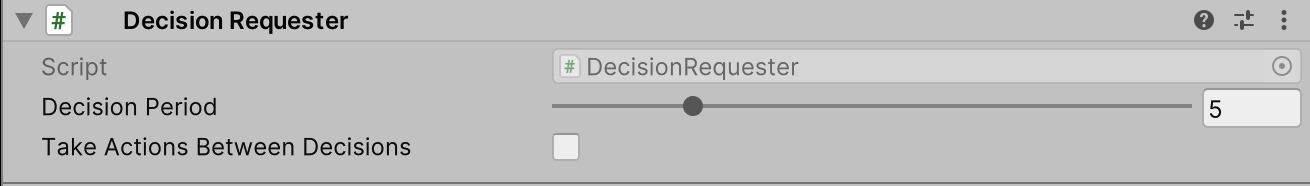
\includegraphics[scale=0.5]{img/entscheidung_anfragen_komponente.png}
  \caption{Unity ML-Agents Entscheidung Anfragen Komponente}
  \label{fig:entscheidung_anfragen_komponente}
\end{figure}

Die Komponente in Abbildung \ref{fig:entscheidung_anfragen_komponente} fragt in regelmäßigen Abständen Entscheidungen an. Das bedeutet es wird eine Beobachtung erstellt. Darauf wird die Beobachtung als Eingangswert für das neuronale Netz genutzt und dann eine Aktion vom neuronalen Netz ausgewählt. Während dem training wird diese Beobachtung zusammen mit der darauf ausgeführten Aktion und der resultierenden Belohnung im Trainingsspeicher abgelegt. Die "Decision Period" gibt an in welchem Interval der Agent eine Entscheidung treffen soll. Das "Kontrollkästchen Take Actions Between Decisions" gibt an ob der Agent die ausgewählte Aktion wiederholen soll bis die nächste Aktion ausgewählt wurde.
